\documentclass[10pt,a4paper]{article}
\usepackage[a4paper,margin=2.1cm,top=2.0cm,bottom=2.2cm]{geometry}
\usepackage{fontspec}
\usepackage{amsmath,amssymb}
\usepackage{tikz}
\usetikzlibrary{arrows.meta,positioning,calc,fit}
\usepackage{fancyvrb}
\usepackage[most]{tcolorbox}
\usepackage{booktabs,array,tabularx}
\usepackage{titlesec}
\usepackage{enumitem}
\usepackage{microtype}
\IfFontExistsTF{Avenir Next}{\setmainfont{Avenir Next}[Ligatures=TeX]}{%
\IfFontExistsTF{Helvetica Neue}{\setmainfont{Helvetica Neue}[Ligatures=TeX]}{%
  \setmainfont{Latin Modern Sans}[Ligatures=TeX]}}
\IfFontExistsTF{Menlo}{\setmonofont{Menlo}[Scale=0.84]}{%
\IfFontExistsTF{DejaVu Sans Mono}{\setmonofont{DejaVu Sans Mono}[Scale=0.84]}{%
  \setmonofont{Latin Modern Mono}}}
\definecolor{ink}{HTML}{1F2933}
\definecolor{soft}{HTML}{52606D}
\definecolor{faint}{HTML}{9AA5B1}
\definecolor{rule}{HTML}{D9DEE4}
\definecolor{wash}{HTML}{F5F7FA}
\definecolor{blue}{HTML}{2B5F9E}
\definecolor{blueL}{HTML}{D6E3F3}
\definecolor{amber}{HTML}{D4881C}
\definecolor{amberL}{HTML}{F9E7C8}
\definecolor{green}{HTML}{1E8A6A}
\definecolor{greenL}{HTML}{D3EDE4}
\definecolor{purple}{HTML}{7B4EA3}
\definecolor{purpleL}{HTML}{E9DFF2}
\definecolor{red}{HTML}{C23B31}
\color{ink}
\setlength\parindent{0pt}
\setlength\parskip{0.55em}
\linespread{1.08}
\titleformat{\section}{\fontsize{14}{17}\selectfont\bfseries}{\thesection}{0.6em}{}
\titlespacing*{\section}{0pt}{1.3em}{0.3em}
\titleformat{\subsection}{\fontsize{8.5}{10}\selectfont\bfseries\color{soft}}{}{0em}{\MakeUppercase}
\titlespacing*{\subsection}{0pt}{0.9em}{0.1em}
\newcommand\code[1]{\texttt{#1}}
\newcommand\file[1]{\texttt{\color{soft}#1}}
\tcbset{codebox/.style={colback=wash,colframe=wash,boxrule=0pt,arc=2.5pt,
  left=6pt,right=6pt,top=3pt,bottom=3pt,before skip=0.6em,after skip=0.6em}}
\newenvironment{rocq}{\VerbatimEnvironment\begin{tcolorbox}[codebox]%
  \begin{Verbatim}[fontsize=\small]}{\end{Verbatim}\end{tcolorbox}}
\tikzset{
  box/.style={draw=#1,fill=#1L,rounded corners=2.5pt,line width=0.6pt,
    inner xsep=6pt,inner ysep=5pt,align=center,font=\small},
  box/.default=blue,
  arr/.style={-{Stealth[length=5pt,width=4pt]},line width=0.6pt,draw=soft},
  lab/.style={font=\footnotesize,text=soft},
}
\pagestyle{plain}
\emergencystretch=4em
\hyphenpenalty=10000 \exhyphenpenalty=10000
\begin{document}

{\fontsize{24}{28}\selectfont\bfseries Names, binding and alpha-equivalence\par}
\vspace{0.2em}
{\large\color{soft} How the Rocq model of Flambda 2 treats them, and how that
compares with nominal sets\par}
\vspace{0.4em}
{\small\color{faint} From the sources of \code{middle\_end/flambda2/rocq/} and
\code{types/rocq/} on the branch \code{flambda2-rocq-semantics}; the
development's own account is \code{NAMES.md} there.\par}
\vspace{0.3em}
{\color{rule}\hrule height 0.6pt}

\section*{In one paragraph}

Terms are ordinary named syntax: a \code{Let} holds a variable and a body, and
nothing is quotiented. Bound names are handled the nominal way: by
\emph{permutations} of names that act on bound and free occurrences alike, so
renaming never captures. Everything else is stated against that action. The
free names, the machine, and (one at a time) every rewrite and check of the
validator are proved to commute with it; alpha-equivalence is an inductive
relation generated by ``permute the bound names''; the comparison that actually
runs is a boolean function proved to coincide with it on well-formed terms; and
an interface copied from the compiler's \code{nominal/} library carries the laws
of a nominal set and of name abstraction. It is nominal sets done as a
\emph{discipline over raw terms}, with the quotient left implicit, about
17,700 lines of statements and proofs in the terms library alone.

\section{The construction}

\subsection{Names and permutations}

Two sorts of name are bound and renamed: variables and continuations. Both are
\code{positive}. Symbols, code ids and slots are global and never move; run-time
values hold no names at all. A permutation is a list of swaps, and a renaming is
one permutation for each sort (\file{FlambdaNominalSpec.v}):

\begin{rocq}
Definition permutation : Type := list (positive * positive).
Fixpoint permute (p : permutation) (name : positive) : positive := ...
Record renaming := Renaming { variable_permutation     : permutation;
                              continuation_permutation : permutation }.
\end{rocq}

A list of swaps is a finite bijection by construction, so there is no
side condition ``$\pi$ is a permutation'' to carry. Two lists that act alike
are identified by \code{same\_permutation}, not by \code{=}. Names are compared
by equality only; the single function that looks at the number of a name is
\code{fresh\_name}, which returns one more than the largest name it is given.

\subsection{The action, and what commutes with it}

\code{rename\_expr r e} applies the renaming to \emph{every} occurrence in
\code{e}, binding or not. It is proved to be a group action
(\file{FlambdaAlphaSpec.v}). The same action is defined on environments,
continuation closures, states, results of a step and behaviours, and the
machine commutes with it unconditionally (\file{FlambdaEquivarianceSpec.v}):

\begin{center}
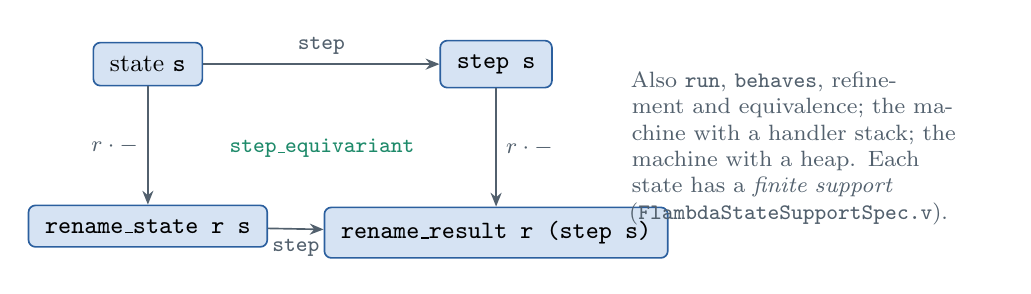
\begin{tikzpicture}[node distance=1.5cm and 3.0cm]
  \node[box] (s) {state \code{s}};
  \node[box,right=of s] (ss) {\code{step s}};
  \node[box,below=of s] (rs) {\code{rename\_state r s}};
  \node[box,below=of ss] (rss) {\code{rename\_result r (step s)}};
  \draw[arr] (s) -- node[lab,above]{\code{step}} (ss);
  \draw[arr] (rs) -- node[lab,below]{\code{step}} (rss);
  \draw[arr] (s) -- node[lab,left]{$r\cdot{-}$} (rs);
  \draw[arr] (ss) -- node[lab,right]{$r\cdot{-}$} (rss);
  \node[lab,text=green] at ($(s)!0.5!(rss)$) {\code{step\_equivariant}};
  \node[lab,right=1.6cm of $(ss)!0.5!(rss)$,text width=4.6cm,align=left]
    {Also \code{run}, \code{behaves}, refinement and equivalence; the machine
     with a handler stack; the machine with a heap. Each state has a
     \emph{finite support} (\file{FlambdaStateSupportSpec.v}).};
\end{tikzpicture}
\end{center}

So a rewrite that is correct for one choice of names is correct for every
other. The same equation, $f(r\cdot e) = r\cdot f(e)$, is then owed by each
function on terms: the free names, the three well-formedness conditions, each
rewrite of the normalisation, each check. These are separate theorems, one per
function, proved by a recursion over terms (\file{FlambdaValidatorEquivarianceSpec.v}
and the Spec file of each pass; the same for typing environments, types, meet
and join in the types library).

\subsection{Alpha-equivalence, three ways}

There are three accounts of ``the same up to bound names'', and theorems that
join them.

\begin{center}
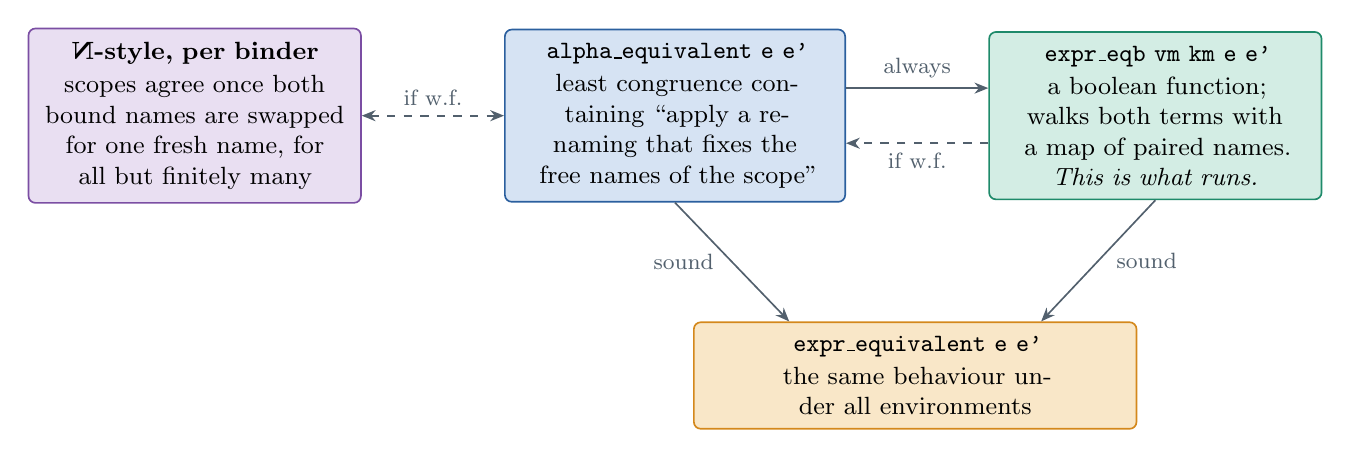
\begin{tikzpicture}
  \node[box=purple,text width=3.8cm,minimum height=2.1cm] (fresh) at (-6.1,0)
    {\textbf{\reflectbox{N}-style, per binder}\\[1pt]
     scopes agree once both bound names are swapped for one fresh name, for
     all but finitely many};
  \node[box,text width=3.9cm,minimum height=2.1cm] (alpha) at (0,0)
    {\textbf{\code{alpha\_equivalent e e'}}\\[1pt]
     least congruence containing ``apply a renaming that fixes the free names
     of the scope''};
  \node[box=green,text width=3.8cm,minimum height=2.1cm] (eqb) at (6.1,0)
    {\textbf{\code{expr\_eqb vm km e e'}}\\[1pt]
     a boolean function; walks both terms with a map of paired names.
     \emph{This is what runs.}};
  \node[box=amber,text width=5.2cm] (sem) at (3.05,-3.3)
    {\textbf{\code{expr\_equivalent e e'}}\\[1pt] the same behaviour under all
     environments};
  \draw[arr] ($(alpha.east)+(0,0.35)$) -- node[lab,above]{always}
    ($(eqb.west)+(0,0.35)$);
  \draw[arr,dashed] ($(eqb.west)+(0,-0.35)$) -- node[lab,below]{if w.f.}
    ($(alpha.east)+(0,-0.35)$);
  \draw[arr,{Stealth[length=5pt,width=4pt]}-{Stealth[length=5pt,width=4pt]},dashed]
    (fresh) -- node[lab,above]{if w.f.} (alpha);
  \draw[arr] (alpha.south) -- node[lab,left,xshift=-3pt]{sound}
    ($(sem.north)+(-1.6,0)$);
  \draw[arr] (eqb.south) -- node[lab,right,xshift=3pt]{sound}
    ($(sem.north)+(1.6,0)$);
\end{tikzpicture}\\[2pt]
{\footnotesize\color{soft} Solid arrows hold of all terms; ``if w.f.'' holds of
terms with distinct binders and closed code, which well-formedness requires.
The theorems, left to right: \code{alpha\_let\_iff} and its siblings;
\code{expr\_eqb\_iff\_alpha\_equivalent}; and below,
\code{alpha\_equivalent\_sound} and \code{expr\_eqb\_sound}.}
\end{center}

The relation has the usual closure rules and one rule per binder; for a
\code{Let} (\file{FlambdaAlphaSpec.v}):

\begin{rocq}
| Alpha_let (r : renaming) x kind defining_expr body :
    code_closed body = true ->
    fixes_names r (without [x] (free_variables_of_expr body))
                  (free_continuations_of_expr body) ->
    alpha_equivalent (Let x kind defining_expr body)
      (Let (rename_variable r x) kind defining_expr (rename_expr r body))
\end{rocq}

The comparison is the primary notion, because it is a function and it is
extracted. At a binder it pairs the two bound names and carries on:
\code{expr\_eqb ((x, x') :: vm) km body body'}. It is proved to be an
equivalence relation, sound for the semantics, invariant under renaming of
both terms, and to accept every alpha-equivalent pair. The converse holds on
terms whose binders are distinct and whose code is closed, which are the terms
well-formedness admits
(\code{expr\_eqb\_iff\_alpha\_equivalent}); outside them the comparison accepts
strictly more, and two counterexamples are proved (a repeated parameter; a
variable bound around open code).

The third account is the one from the literature, recovered as a theorem at
each binder. For a \code{Let} it is in \file{FlambdaCompareConverseSpec.v}; the
other binders are in \file{FlambdaAlphaFreshSpec.v} and
\file{FlambdaAlphaGroupSpec.v}.

\begin{rocq}
alpha_equivalent (Let x kind d body) (Let x' kind' d' body')
<-> kind = kind' ∧ d = d'
    ∧ И fresh, alpha_equivalent (rename_expr (swap_variable x  fresh) body)
                                (rename_expr (swap_variable x' fresh) body')
\end{rocq}

where \code{И x, P x} is defined as $\exists$ a finite list to avoid,
$\forall$ names outside it, \code{P} (\file{FlambdaFreshQuantifierSpec.v}).

\newpage
\subsection{The interface: things that contain names, and abstractions}

\file{FlambdaNameAbstractionSpec.v} transcribes three signatures of the
compiler's \code{nominal/} library, \code{Contains\_names}, \code{Bindable} and
\code{Name\_abstraction}, and adds the laws that the OCaml leaves unsaid:

\begin{rocq}
Record contains_names (T : Type) := {
  apply_renaming : permutation -> T -> T;
  free_names     : T -> list positive;
  equal          : T -> T -> Prop }.

Record nominal (N : contains_names T) : Prop := {
  (* equal is an equivalence; the action is a group action that     *)
  (* respects same_permutation and equal;                           *)
  free_names_equivariant : among (permute p n) (free_names (p · t))
                           = among n (free_names t);
  free_names_equal       : equal t t' -> same_names (free_names t) (free_names t');
  apply_renaming_fixes   : fixes p (free_names t) -> equal (p · t) t }.
\end{rocq}

A name abstraction is a pair \code{\{bound : B; scope : T\}} where \code{B} is
\emph{bindable} (a name, or a list of names). It is opened by
\code{pattern\_match p a}, which renames both parts with a permutation that
fixes the free names of the abstraction. Two abstractions are equal when they
can be opened to the same bound names and equal scopes:

\begin{center}
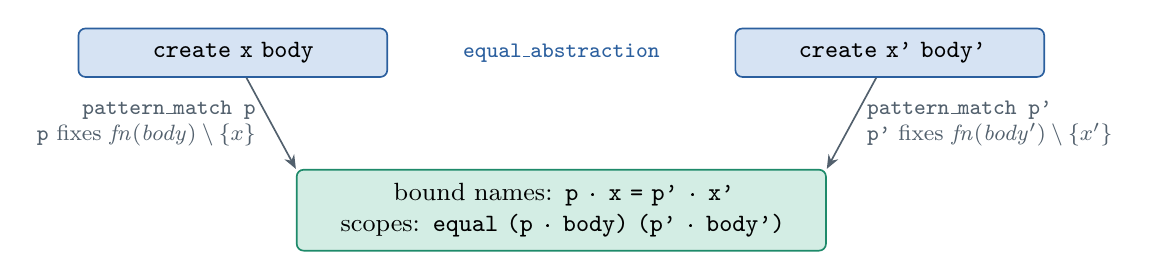
\begin{tikzpicture}[node distance=0.9cm and 1.0cm]
  \node[box,text width=3.5cm] (a) {\code{create x body}};
  \node[box,text width=3.5cm,right=4.4cm of a] (b) {\code{create x' body'}};
  \node[box=green,text width=6.3cm] (c) at ($(a)!0.5!(b)+(0,-2.0)$)
    {bound names: \code{p · x = p' · x'}\\
     scopes: \code{equal (p · body) (p' · body')}};
  \draw[arr] (a) -- node[lab,left,align=right,xshift=-2pt]
    {\code{pattern\_match p}\\ \code{p} fixes $\mathit{fn}(\mathit{body})\setminus\{x\}$} (c.north west);
  \draw[arr] (b) -- node[lab,right,align=left,xshift=2pt]
    {\code{pattern\_match p'}\\ \code{p'} fixes $\mathit{fn}(\mathit{body'})\setminus\{x'\}$} (c.north east);
  \node[lab,text=blue] at ($(a)!0.5!(b)$) {\code{equal\_abstraction}};
\end{tikzpicture}
\end{center}

Abstractions of a nominal type by a bindable one are again nominal
(\code{abstraction\_nominal}), opening does not depend on the permutation
chosen (\code{pattern\_match\_pair}, \code{pattern\_match\_well\_defined}), and
for a single bound name the definition is equivalent to the
\reflectbox{N}-form (\code{equal\_abstraction\_fresh}).
Then the terms are connected to the interface: \code{simple}, \code{named},
static constants and environments are instances with \code{equal := eq};
expressions with closed code are an instance, per sort, with \code{equal :=
alpha\_equivalent}; and each binder (\code{Let}, \code{Let\_cont}, handler,
code, recursive group) is shown to \emph{be} a name abstraction, in the sense
that equal abstractions give alpha-equivalent terms
(\file{FlambdaNominalInstancesSpec.v}).

\subsection{Functions that make names}

No function that picks a fresh name commutes with every renaming
(\code{no\_source\_commutes}): if the source answers $n$ for a list $l$, swap
$n$ with some $y \notin l$; the list is unchanged, so the source still answers
$n$, but the renamed answer is $y$. A rewrite that leaves a made name in its
result therefore cannot satisfy $f(r\cdot e) = r\cdot f(e)$. Two replacements
are used:

\begin{itemize}[leftmargin=1.2em,itemsep=0.2em,topsep=0.2em]
\item \textbf{Up to the names made.} \code{equivariant\_up\_to f}: on closed
  code, $f(r\cdot e) = r'\cdot f(e)$ for some $r'$ that agrees with $r$ on the
  free names of $f(e)$. With \code{keeps\_scope} (no new free names) this
  composes and iterates, and \code{expr\_eqb} cannot tell the results apart.
  \code{rename\_apart} and inlining at fresh names are stated this way.
\item \textbf{With the source renamed.} The source is an argument, and a
  renaming acts on it by conjugation, \code{rename\_fresh r fresh := fun l =>
  r · fresh (r⁻¹ · l)}. The function then satisfies the plain equation with
  the renamed source. The join of typing environments, whose made variables
  stay free in its answer, is stated this way.
\end{itemize}

\section{Comparison with nominal sets}

The reference points are Gabbay and Pitts [1,2], Pitts's nominal logic [3] and
book [5], alpha-structural recursion [4], and the two mechanisations closest
in spirit: Nominal Isabelle [6,7] and Aydemir, Bohannon and Weirich's nominal
techniques in Coq [8].

\subsection{What is the same}

{\small
\renewcommand\arraystretch{1.35}
\begin{tabularx}{\linewidth}{@{}>{\raggedright\arraybackslash}p{3.3cm}>{\raggedright\arraybackslash}X>{\raggedright\arraybackslash}X@{}}
\toprule
& \textbf{Nominal sets} & \textbf{The Rocq development} \\
\midrule
Atoms & A countably infinite set $\mathbb{A}$, possibly sorted; only equality
  is observable & \code{positive}, two sorts; ``compared by equality only'' is a
  stated rule, with one exception (\code{fresh\_name}) \\
Permutations & $\mathrm{Perm}(\mathbb{A})$: finite permutations & Lists of
  swaps, identified extensionally. The same representation as Nominal
  Isabelle~[6] \\
Carrier & A set with a $\mathrm{Perm}$-action in which every element has a
  finite support & \code{contains\_names} + \code{nominal}: an action, a
  finite list \code{free\_names}, and the law that a permutation fixing it
  fixes the element \\
Support & $\mathrm{supp}(x)$, the \emph{least} finite support; a derived
  notion & \code{free\_names} is \emph{given}. Minimality is not a law, but it
  follows: see below \\
Freshness $a \mathrel{\#} x$ & $a \notin \mathrm{supp}(x)$ &
  \code{among a (free\_names x) = false} \\
Equivariant map & $f(\pi\cdot x) = \pi\cdot f(x)$; has
  $\mathrm{supp}(f\,x)\subseteq\mathrm{supp}(x)$ & \code{equivariant};
  \code{invents\_no\_names} is exactly that inclusion \\
Abstraction $[\mathbb{A}]X$ & $(a,x)\sim(a',x')$ iff
  $(a\;c)\cdot x = (a'\;c)\cdot x'$ for some/any fresh $c$ &
  \code{name\_abstraction}; equality by permutations that open both, proved
  equivalent to the fresh-name form, with both the ``some'' and the ``any''
  reading \\
\reflectbox{N} quantifier & ``for all but finitely many $a$'' & \code{for\_fresh},
  with notation \code{И}; a derived view, not a primitive \\
Binding several names & Generalised abstraction; Nominal2's binders of lists
  and sets~[7] & \code{bindable}: \code{single\_name}, \code{list\_of\_names};
  parameters, recursive groups, the four names of code \\
\bottomrule
\end{tabularx}}

Two of these deserve a remark. First, the laws of \code{nominal} do pin
\code{free\_names} down to the least support, although no law says so: if $S$
supports $t$ and $a \in \mathit{fn}(t)\setminus S$, swap $a$ with a fresh
$b$; the swap fixes $S$, so the result is \code{equal} to $t$ and has the same
free names, yet by equivariance of \code{free\_names} it contains $b$. This is
the argument behind \code{invents\_no\_names}. Second, the definition of equal
abstractions by a permutation that fixes the free names of the abstraction is
the one Urban and Kaliszyk use for general binders~[7], made symmetric.

\subsection{What is different}

\textbf{No quotient.} A nominal datatype \emph{is} the set of alpha-classes: in
[1,2] and in Nominal Isabelle, $\lambda a.t$ is built with the abstraction
former and $\lambda a.a = \lambda b.b$ is an equation. Here \code{expr} is raw
syntax and \code{Let x} $\neq$ \code{Let y} as terms. The nominal set is the
setoid (\code{expr} with closed code, \code{alpha\_equivalent}); the instance
theorem says so, and the ``binder is an abstraction'' theorems say that the
constructors behave as the abstraction former would. This is the route of
Aydemir et al.~[8], whose Coq records of an action, a support and their laws
are close to \code{contains\_names}. The price is that every function on terms
owes a proof that it respects alpha-equivalence or commutes with renaming; the
benefit is that the functions are ordinary structural recursions that extract
to the OCaml one would write.

\textbf{No alpha-structural recursion.} Pitts's recursion principle~[4] lets a
function be defined on classes by giving its action on a binder with a fresh
name, subject to the \emph{freshness condition for binders}: the bound name is
not in the support of the result. The development has no such principle, but
the same condition appears as the premise of
\code{pattern\_match\_well\_defined} (``no bound name is free in its
result''), which says when a function of an opened abstraction is independent
of how it was opened. It is the correctness condition for the compiler's
\code{pattern\_match}, stated but not turned into a way of defining functions.

\textbf{Equivariance is proved, not inherited.} In nominal logic everything
definable is equivariant~[3], and Nominal Isabelle derives equivariance lemmas
automatically. Here each function has its own theorem (the table in
\code{NAMES.md} runs to dozens of files). That is partly the cost of working in
plain Rocq, and partly a feature: the functions model compiler code, and a
function whose answer depends on the order of names is a real bug that such a
theorem would refuse (the document records several places where the compiler
falls back on the order of stamps).

\textbf{A decision procedure is primary.} The literature defines
alpha-equivalence and derives algorithms; here \code{expr\_eqb} comes first,
because it is extracted and run, and the relation is a set of facts about it.
The comparison is not the nominal one (open both sides at one fresh name, as
the compiler's \code{pattern\_match\_pair} does) but the environment-of-pairs
one familiar from locally-nameless and de Bruijn-level checkers. The two are
proved to agree only under \code{binders\_distinct} and \code{code\_closed}.

\textbf{Name generation leaves the category.} Nominal sets handle fresh names
by never choosing one: \reflectbox{N}, or a freshness theorem that needs the
name not to escape. The standard fact that there is no equivariant choice of
an atom is \code{no\_source\_commutes}. The development needs deterministic,
extractable functions, so it chooses anyway and repairs the statement.
\code{equivariant\_up\_to} with \code{keeps\_scope} amounts to equivariance on
alpha-classes when the made names are bound in the result. The second repair,
acting on the source by conjugation, uses the nominal action on functions,
$(\pi\cdot f)(x) = \pi\cdot f(\pi^{-1}\cdot x)$, but on a function that has
\emph{no finite support} (the swapping argument above works against any
finite $S$). Such a function is not an element of a nominal function space;
the equations hold in the larger world of sets with a permutation action.
That is harmless for the theorems, but it means the literature's results about
finitely supported functions do not apply to the join as stated.

\textbf{Restrictions that come from Flambda.} Every rule that renames a binder
carries \code{code\_closed}: code is a binder for all names (its body may
mention only its own parameters), and the comparison assumes it. Nominal
syntax has no counterpart; it is an invariant of the language, not of the
method. Likewise the interface is one sort at a time, while the machine is
renamed in both sorts at once, so states are shown to be finitely supported
directly and are not instances of \code{nominal}. Heap locations are a third
sort whose permutations are not yet defined.

\subsection{Summary}

\begin{tcbraster}[raster columns=3,raster equal height,raster column skip=8pt,
  boxrule=0.6pt,arc=2.5pt,left=7pt,right=7pt,top=5pt,bottom=5pt,
  fontupper=\footnotesize,before skip=0.6em,after skip=0.8em]
\begin{tcolorbox}[colback=blueL,colframe=blue]
{\small\textbf{Taken from nominal sets}}\par\smallskip
permutations, not substitutions\par equivariance as the basic law\par
finite support\par abstraction, generalised binders\par
the \reflectbox{N} quantifier
\end{tcolorbox}
\begin{tcolorbox}[colback=amberL,colframe=amber]
{\small\textbf{Done differently}}\par\smallskip
raw terms; a setoid, not a quotient\par
support given as data (\code{free\_names})\par
equivariance proved per function\par
a boolean comparison comes first\par
fresh names chosen, then repaired
\end{tcolorbox}
\begin{tcolorbox}[colback=purpleL,colframe=purple]
{\small\textbf{Not there}}\par\smallskip
alpha-structural recursion, induction\par
equivariance for free\par
finitely supported function spaces\par
an interface for two sorts at once\par
permutations of heap locations
\end{tcolorbox}
\end{tcbraster}

The gap that would matter most for future proofs is the second column's first
line together with the third column's first: without an induction principle
that lets bound names be assumed fresh, each proof by cases on terms handles
renaming by hand, which is likely where much of the size of the
\code{*Equivariance*} and \code{*Scope*} files comes from. Nominal Isabelle's answer is strong induction
with a freshness context; a Rocq analogue over \code{expr} (induction up to
\code{alpha\_equivalent}, with the bound names of each case outside a given
finite list) looks derivable from what is already proved, since
\code{rename\_apart} and the binder-as-abstraction theorems are in place; I
have not tried it.

\vspace{0.4em}
{\color{rule}\hrule height 0.6pt}
\vspace{0.3em}
{\footnotesize\color{soft}
\begin{enumerate}[label={[\arabic*]},leftmargin=2em,itemsep=0.05em,topsep=0.2em]
\item M. J. Gabbay and A. M. Pitts. A new approach to abstract syntax involving binders. \emph{LICS}, 1999.
\item M. J. Gabbay and A. M. Pitts. A new approach to abstract syntax with variable binding. \emph{Formal Aspects of Computing} 13, 2002.
\item A. M. Pitts. Nominal logic, a first order theory of names and binding. \emph{Information and Computation} 186, 2003.
\item A. M. Pitts. Alpha-structural recursion and induction. \emph{Journal of the ACM} 53, 2006.
\item A. M. Pitts. \emph{Nominal Sets: Names and Symmetry in Computer Science}. Cambridge University Press, 2013.
\item C. Urban. Nominal techniques in Isabelle/HOL. \emph{Journal of Automated Reasoning} 40, 2008.
\item C. Urban and C. Kaliszyk. General bindings and alpha-equivalence in Nominal Isabelle. \emph{ESOP}, 2011.
\item B. Aydemir, A. Bohannon and S. Weirich. Nominal reasoning techniques in Coq. \emph{LFMTP}, 2006.
\end{enumerate}
The citations are from memory and were not checked against the papers; the
claims about the development were checked against its sources and
\code{NAMES.md}, not by building it.}

\end{document}
